\documentclass[a4paper,12pt]{article}
\usepackage{graphicx}
\usepackage{amsmath, amsfonts}
\usepackage{amssymb}

\usepackage[utf8x]{inputenc}
\usepackage[T1]{fontenc}

\usepackage{lmodern}
\usepackage{textcomp}

\usepackage{natbib}

\usepackage[top=1.2in,bottom=1.2in,left=3.cm,right=3.cm,a4paper]{geometry}

\usepackage[font=footnotesize]{caption}

\usepackage{xcolor}

%\usepackage{hyperref}

%\hypersetup{
%    colorlinks,
%    linkcolor={red!50!black},
%    citecolor={blue!50!black},
%    urlcolor={blue!99!black}
%}

\usepackage{titling}
\usepackage{ragged2e}




\usepackage[nottoc,numbib]{tocbibind}

%%%%%%%%%%%%%%%%%%%%%%%%%%%%%%%%%%%%%%%%%%%%%%%%%%%%%%%%


% to define new commands
%\newcommand{\R}{\mathcal{R}}
%\newcommand{\mean}[1]{\langle #1 \rangle}

% to show the pieces of advice
%\newcommand{\advice}[1]{{\it #1}}
% to hide the pieces of advice
% \newcommand{\advice}[1]{}

\begin{document}

\begin{center}
	
	\begin{figure} [t]
		
\includegraphics[width=0.3\linewidth]{../fig/logo_UGA.png}
		\hspace{5.0cm}
		
\includegraphics[width=0.3\linewidth]{../fig/logo_IGE.png}
		\vspace{2.0cm}
	\end{figure}
	
	\begin{Large}
		\textbf{Numerical experiments of glacial inceptions in Northern Europe}
	\end{Large}
	
	\vspace{0.4cm}
	
	\textbf{ESPELETA BOLIVAR, Ruben Dario}
	
	\vspace{3.0cm}
	
	
	\textbf{Research project}\\
	Presented in partial fulfillment of the requirements for the degree of\\
	\textbf{Master applied mechanics}\\
	
	
	\vspace{3.0cm}
	
	Université Grenoble Alpes\\
	\textbf{\today}
	\vspace{4.0cm}
	
\end{center}

\flushleft{
	Project Advisor(s):\\
	Cruz Garcia Molina
}
\renewcommand{\labelitemi}{$\bullet$}


\tableofcontents

\newpage
\begin{abstract}
	\justifying
	In response to the perturbation of global climate systems, such as climate change, glaciars are losing mass. This mass loss has had consequences on sea level rise, but also on the climate system itself as a whole through different phenomena. 
	
	The present project's aim is to perform numerical simulations using the Finite element method Elmer/Ice. The impact of the variation of different parameters that are involved in idealised tophography ice sheet flows will be studied. These results will help us to better understand the behiavor and the importance that these parameters have on Northern Europe ice sheets dynamics. Through these analysis of idealised cases in the present project, we aim to understand the behavior in more realistic scenarios of past and present glacial inceptions in Northern Europe. 
\end{abstract}
\pagebreak

\section{Introduction}
\justifying
As Earth's largest reservoirs of fresh water, ice sheets are important components of the global climate system \cite[]{zhang2017comparison}. The impacts of the perturbation of these climate systems are most acutely changes in global see level, as ice sheets grow or decay in response to climate forcing and internally controlled dynamics. While the rate of present-day sea-level rise is dominated by ocean steric changes and eustatic changes due to shrinking mountain glaciers, the eustatic contribution from the large ice sheets (Greenland and Antartic) has increased in recent decades and it is expected to continue increasing in coming decades and centuries \cite[]{clark2015recent}. To have a better idea, if all the ice were to melt completely, the sea level would rise by an estimated 65m \cite[]{morlighem2017bedmachine,haywood2011pliocene} and force populations to emigrate their land submerged by water.

In order to understand these impacts on the dynamics and melting of ice sheets and glaciers, numerical models are developped. Through these models, some of them which are based on finite elements, we can have simulations that can make better predictions of future ice sheets behaviour and rate of sea level rise, and ultimately provide policy makers with improved estimates of future change.

\begin{figure}[!h]
	\centering
	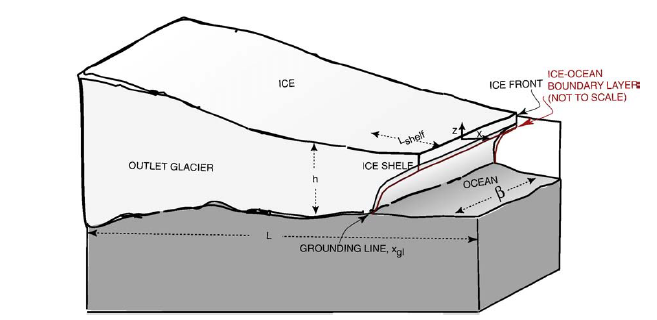
\includegraphics[width=0.7\linewidth]{../fig/Scheme_grounding_line}
	\caption{Schematic simplified diagram of the model domain of a glacier \cite[]{parizek2010implications}.}
	\label{groundingline}
\end{figure}

There are different parameters and variables that affect the ice sheet melting, and that play an important role in the dynamics of the glaciers. One of this important parameters is the grounding line, and its location is still topic of discussion in the literature surrounding ice sheets dynamics \cite[]{goldberg2018representing}.

Glaciers that end in the ocean are called tidewater glaciers. Glaciers that flow into an ice shelf are called tributary glaciers as the one shown in figure \ref{groundingline} by \cite{parizek2010implications}. The line that divides the part of the glacier that is in contact with the solid bedrock and the ice shelf floating on water driven by buoyancy, is called the grounding line \cite[]{cheng2019full}. The location of the grounding line is important, because mass loss from glaciers is strongly linked to changes in the ice shelves and their grounding lines \cite[]{brunt2010mapping,pritchard2012antarctic}. Its long-term horizontal position is very susceptible to temporal and spacial changes in ice thickness and sea level, as well as bedrock and ice surface slopes. Ice thinning and rising sea level can cause grounding lines to retreat, while thickening or declining sea levels can cause an advance \cite[]{friedl2020remote}. It is important to know the grounding line position to be able to quantify the ice discharge into the sea and as an indicator if the ice sheet is advancing or retreating \cite[]{konrad2018net}.

Grounding lines are actually more of a zone. The grounding zone is the region where ice transitions from grounded ice sheet to freely flotating ice shelf, typically over several kilometers. The grounding zone is the region between point F on figure \ref{groundingzone} by \cite{fricker2009mapping}, where there is no tidal movement, and point H, which is the seaward limit of ice flexure, where the ice is free-floating. The floating ice shelf changes in elevation in response to tides, atmospheric air, pressure and oceanic processes. Grounding occurs when the ice shelf comes into contact with the bedrock below \cite[]{fricker2009mapping}. The transition from grounded ice sheets to flotating ice shelf plays an important role in controlling marine ice sheet dynamics, as it determines the rate at which ice flows out of the grounded part of the ice sheet \cite[]{schoof2007ice}. This is because ice flux through the grounding line increases sharply with ice thickness at the grounding line. This means that grounding lines are unstable on reverse-bed slopes, such as those under Pine island glacier, because recession into deeper water increases ice flux and further encourages more glacier recession \cite[]{schoof2007marine}.

\begin{figure}[!h]
	\centering
	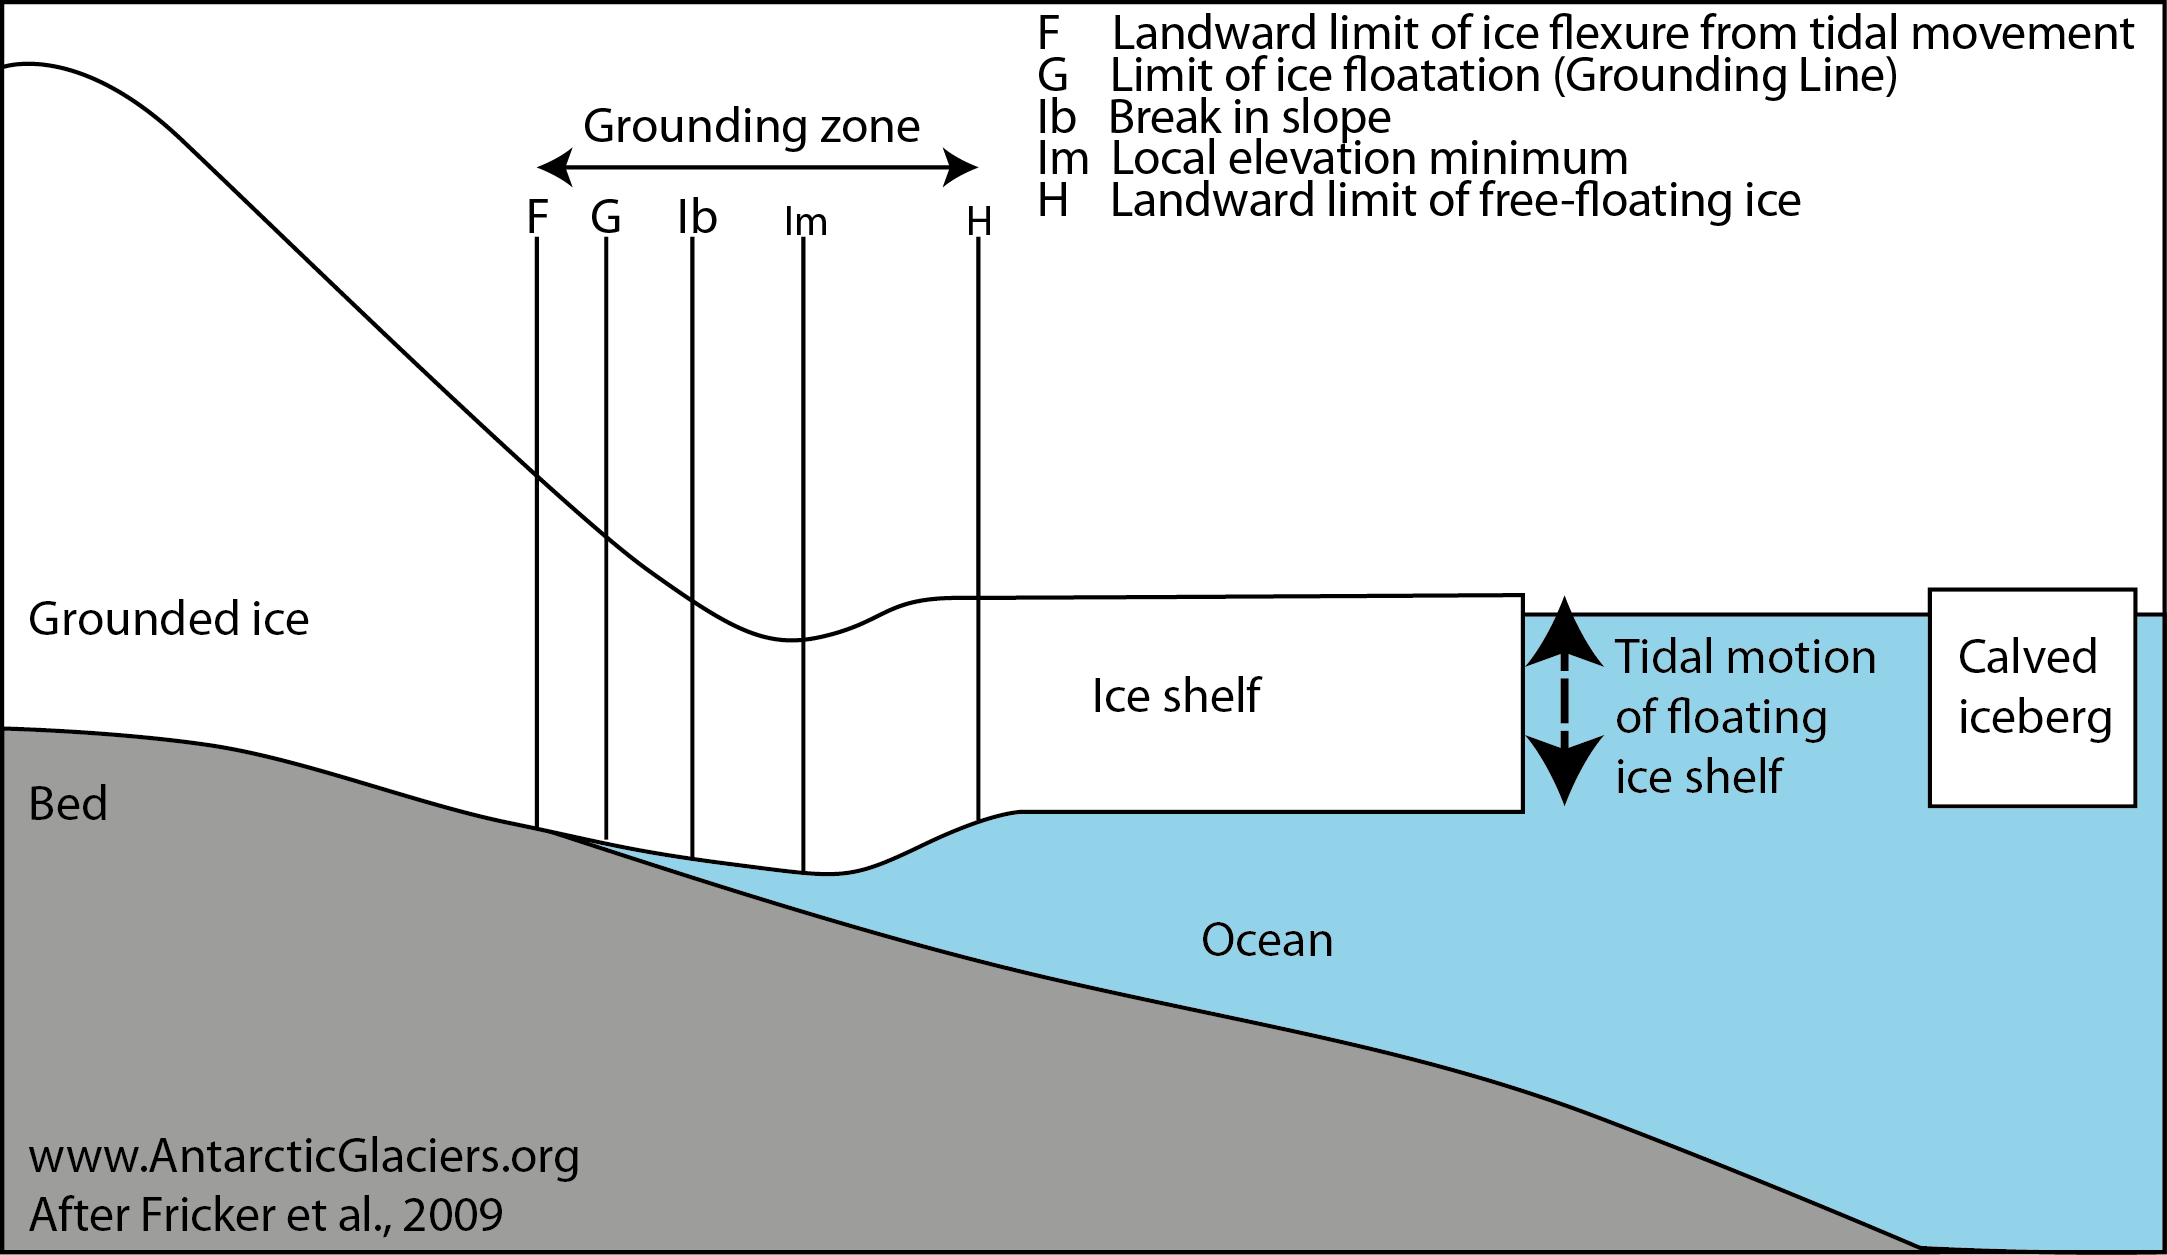
\includegraphics[width=0.7\linewidth]{../fig/groundingzone}
	\caption{Schematic of a tributary glacier where we can observe the different parts denoting the grounding zone \cite[]{fricker2009mapping}.}
	\label{groundingzone}
\end{figure}

During this project, the main objective is to understand the direct impact of changes in the position of the grounding line on the flow dynamics of ice sheets glaciers. For this purpose, we will use the finite element model Elmer/Ice as a simulation tool, which will be presented in this paper. The purpose consists in using different spatial resolutions to compare the changes in the position of the grounding line for different idealised topographies of Northern Europe glaciers. This way, we will test the capability of this numerical model to predict the position of the grounding line in these idealised cases. This will help us to understand the behavior of Northern glaciers ice sheets. 

\section{State of the art}
\subsection{Physical properties of the glaciars}
\subsubsection{Mass and movement balance equations}
An ice sheet is a continuous sheet of land ice that covers a very large aream of several thousands to millions of squared meters. It is formed by an accumulation of snow which will densify under its own weight, until it becomes ice. This ice will then flow downhill under its weight, and can eventually reach the sea. If it does, and the ice propagates above the sea, this part of the ice sheet is called and ice shelf \cite[]{hutter1982mathematical}. The figure \ref{groundingline} shows a diagram of an ice sheet showing different parts of it, such as the ice shelf, and some phenomena happening inside of it, such as the ice flow or the snow accumulation.

The ice is considered as a very viscous fluid, flowing on large time scales. The ice flow equations are then derived from the Stokes equation \cite[]{hutter1982mathematical}:
\begin{equation}
	div\sigma + \rho g = div\tau - gradp + \rho g = 0;
\end{equation}
with $\sigma$ the stress tensor, $\rho$ the density of the ice, g the gravity vector, $\tau$ the deviatoric stress tensor, with $\sigma = \tau - pI$ and $p=\frac{tr\sigma}{3}$. 

And the mass conservation:
\begin{equation}
	\frac{dh}{dt}+ div(uH)=M_s + M_b;
\end{equation}
With $u$ the velocity, H the ice thickness, $M_s$ and $M_b$ the mass balance at the surface and at the bottom respectively. $M_s$ will be defined, and $M_b$ is considered as 0 for convenience purposes. 

The stresses are related to the viscosity and the strain by the Glen's law \cite[]{glen1958flow}:
\begin{equation}
	\tau = 2\eta\dot{\epsilon}
\end{equation}
With the viscosity that can be inferred according to \cite{gagliardini2013capabilities} as:
\begin{equation}
	\eta = \frac{1}{2}(EA)^\frac{-1}{n} \dot{\epsilon_e}^\frac{(1-n)}{n};
\end{equation}
Where:
\begin{itemize}
	\item The strain rate $\dot{\epsilon}$;
	\item Glen's constant n=3;
	\item The enhancement factor to account for an anisotropic effect E=1;
	\item The rheological parameter A=15,46;
\end{itemize}
For an ice sheet, the ratio of the vertical lenght over the horizontal lenght is a little more than $\frac{1}{10^3}$. Indeed, the thickness of an ice sheet is comprised between 0 to a few thousands of meters (e.g. the ice sheet in Greenland is 3300 m thick at most \cite[]{bamber2001new}) and typical horizontal lenght of an ice sheet is of the order of magnitude of 1000 km. This allows simplifications in the equations. One of them is the shallow ice approximation. It assumes a large ratio of horizontal to vertical lenght, that the basal shear stress is balanced by  the gravitational driving stress, and a large vertical to horizontal stress ratio. That represents a slow flow in the interior of an ice sheet (blue regions in Figure \ref{velocityglaciar}). The approximation makes the method computationally cheap and works well over long simulations.

\begin{figure}[!h]
	\centering
	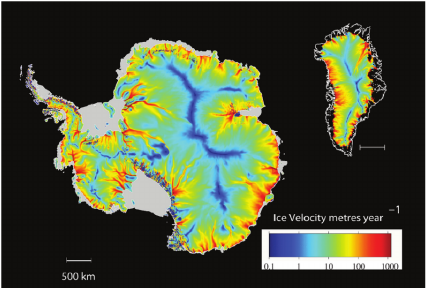
\includegraphics[width=0.7\linewidth]{../fig/velocityglaciar}
	\caption{Ice velocities in Antarctica and Greenland topographies, where we can see in red the highest velocity profiles in the glaciars and as consequence we consider the basal shear stress as 0 and the longitudinal stress dominates, which allows to use a Shallow Shelf approximation \cite[]{allison2009ice}.}
	\label{velocityglaciar}
\end{figure}
Figure \ref{velocityglaciar} shows a map of velocities in Antarctica and Greenland topographies. Where this velocity is the highest, the basal shear stress cannot be considered as balanced by the gravity anymore. Instead, it is taken as 0 and the longitudinal stress dominates. This is the Shallow Shelf approximation, initially developed for ice shelves, but which has been extended to dragging ice streams. It is a 2D vertically integrated model, the ice velocity being depth-averaged.

But these approximations are not mandatory: the Full Stokes model is still the most precise, it accounts for all nine stress components. It is useful around the parts that are at the limits of the others models or over complex topographies, but not needed for the interior of ice sheets, where the improvement would be minimal but the computational cost way higher \cite[]{larour2012continental}.

The factors such as sensitivity, long time intervals, and long distances require a careful treatment of the groundline neighborhood by the numerical method to discretize the model equations \cite[]{cheng2019full}. The most accurate ice model is the Full stokes (FS) equations \cite{cheng2019full}. However, a simplification of these FS equations by integrating in the depth of the ice is the shallow shelf approximation \cite[]{macayeal1989large}.The computational advantage with Shallow Shelf approximation is that the dimension of the problem is reduced by one, it is often used for simulations of the interaction between a grounded ice sheet and a marine ice shelf \cite[]{cheng2019full}. 
In this project, only the Shallow Shelf approximation is made, as this is how future projections of Greenland and Antarctica are done with the Elmer/Ice model.

\subsection{Research background}
A long debate on the dynamics of such ice sheets was initiated in the 1970s, when \cite{weertman1974stability} proposed that a marine ice sheet which lies on an upward-sloping bed is unstable. Recently, the instability hypothesis has been strongly reinforced, based on a boundary-layer theory due to \cite{schoof2007ice}. Moreover, \cite{vieli2005assessing} showed that the poor ability of marine ice-sheet models to give consistent prognostic results and, more particularly, they highlighted the influence of the grid size on model results. One of their main conclusions was that no reliable model was able to predict grounding line dynamics at the time of their study.

As a consequence, there is an urgent need to improve marine ice-sheets models in order to corroborate recent theoretical predictions, and to obtain confident simulations of the grounding line dynamics. \cite{durand2009marine} recently proposed a full stokes resolution of the ice-sheet/ice-shelf transition. This approach has been built on literature dealing with the coupling between a grounded ice sheet and a floating ice shelf and identyfing this transition zone as a crucial control of the marine ice sheet dynamics \cite[]{weertman1974stability,van1985response,chugunov1996modelling,hindmarsh1996stability,vieli2005assessing,schoof2007ice,schoof2007marine}.

Also, \cite{durand2009full} showed, using the finite element code Elmer, that the full stokes modeling of the ice-sheet/ice-shelf transition they proposed can give consistent predictions of grounding-line migration, and that their approach is highly sensitive to the chosen mesh resolution. However, in their results with a grid size down $<5 km$ in the vicinity of the grounding line, predictions start to be robust because: whatever the grid size($<5km$) the steady-state grounding line position is sensibly the same (6km the standart deviation), and with a grid-size refinement in the vicinity of the grounding line (200m), the steady state solution is independent of the applied perturbation in fluidity, provided this perturbation remains monotonic.

In order to study and to test the behavior of the different components of the models, idealized systems are studied and, based on the results that are obtained from these idealised cases, the hypothesis, models and numerical methods used to solve the problems are improved. For this reason, within the framework of this project we will analyze the behiavor of the Elmer/Ice method to solve idealised systems and tophographies. The framework in which the present project is focused, is on the study of the Northern Europe glaciar. But, since this glaciar does not exist anymore, idealised cases simulations of North Europe glaciars, such as Greenland can be analized as mentioned before, and their results can be used to improved the numerical models, hyphotesis and/or parameters of the models, and this way we can better understand the behavior of ancient glaciars such as the Northern Europe glaciar.

\section{Numerical model}
\subsection{The Elmer/Ice finite element method}
In order to model ice sheets, both finite difference method (FDM) and finite element method (FEM) are used (e.g. ISSM (https://issm.jpl.nasa.gov/) and Elmer/ice). Those are numerical methods, since most of the time analytical solutions are challenging, or even impossible to obtain. Finite Difference Method consists in converting ordinary and partial differential equations into a system of linear equations by approximating derivatives as finite differences. Elmer/Ice, on the other hand, uses the Finite Element Method.

Elmer is an open source, parallel, Finite element code, mainly depeloped by the CSC in Finland. The ice sheet/ice flow model Elmer/ice is based on Elmer and includes developments related to glaciological problems. Elmer/ice includes a large number of dedicated solvers and users functions.
Elmer/ice solves the full-stokes equations for various ice rheologies (classical  Glen's flow law, anisotropic laws and porous compressible firns/snow law). It includes solvers for the classical asymptotical expansions of the stokes equations, namely the shallow 	ice approximation (SIA) and the shallow shelf approximation (SSA). All these equations can be solved diagnostically or in transient, allowing the displacement of the boundaries. 

It considers a continuum as an assembly of non-overlapping elements forming the same geometry, which makes the modeling of complex geometries possible. Each element is made of at least two points, on which are applied the forces and computed the displacements. To solve the equations, Elmer/Ice uses subroutines, or solvers. To each equation corresponds one solver to be referenced in the input file, together with the different parameters of the problem. They each compute the evolution of given variables, such as the ice thickness or the velocity, to give at each time step a picture of the flow. All combined, it allows to visualise the evolution of the flow through time.
\section{Model application}

Using different space resolutions on idealised topographies, we will use an idealised system starting from a simple mountain, which work was carried out by last year intern \cite{Dainche2022}, and the parameters and all idealised topographies will be the ones set up in the experiments performed in the model comparation work CalvingIMP, that will be explained in next section. 

In order to model our idealised systems using Elmer/Ice, we start from having a configuration with no ice until having a glaciar in the tophography, and we are interested in analyzing how the results vary as a function of the change in parameters, such as the spacial resolution. We will vary the resolution parameter starting from 10 km, then 5km, 1km and 500m. These results obtained from these simulations will help us understand the assumptions and considerations we need to take into account for further simulations of more realistic topographies where we can include the evolution in time of the sea shore of the last  glaciar inception in the Northern Europe.

\subsection{Numerical setup}
\subsubsection{Bedrock and topography}
The idealised model consists of a circular bedrock configuration $Bed$ (Figure \ref{circular_topo_top} and Figure \ref{circular_topo_jet}) given by:
\begin{equation}
	\theta=arctan2(y,x);
\end{equation}
\begin{equation}
	I=R-cos(2\theta)\frac{R}{2}
\end{equation}
\begin{equation}
	Bed_0=Bc-(Bc-BI)\frac{|x^2+y^2|}{R2}^;
\end{equation}
Where $R=800x10^3 m$, $Bc=0.9 x 10^3 m$, and $BI=-2 x 10^3 m$. 
\begin{figure}[!h]
	\centering
	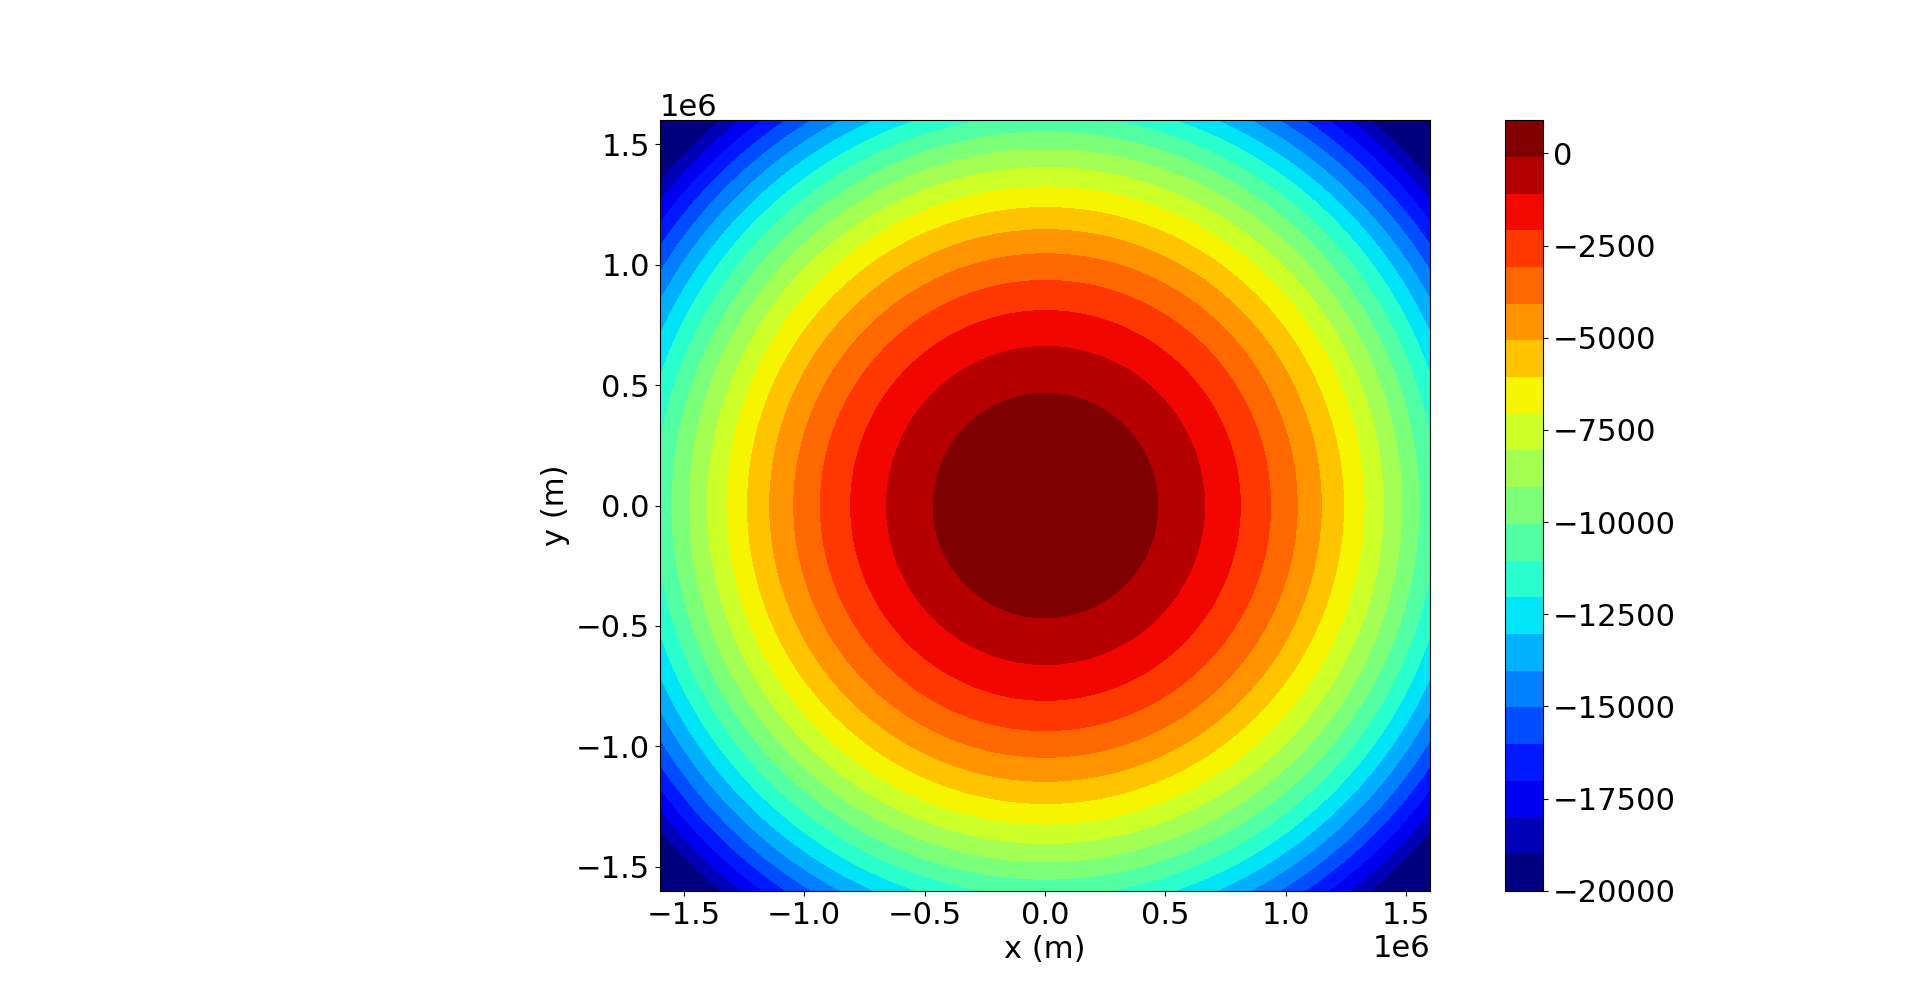
\includegraphics[width=0.7\linewidth]{../fig/circular_topo_top}
	\caption{Circular bedrock top view.}
	\label{circular_topo_top}
\end{figure}
\begin{figure}[!h]
	\centering
	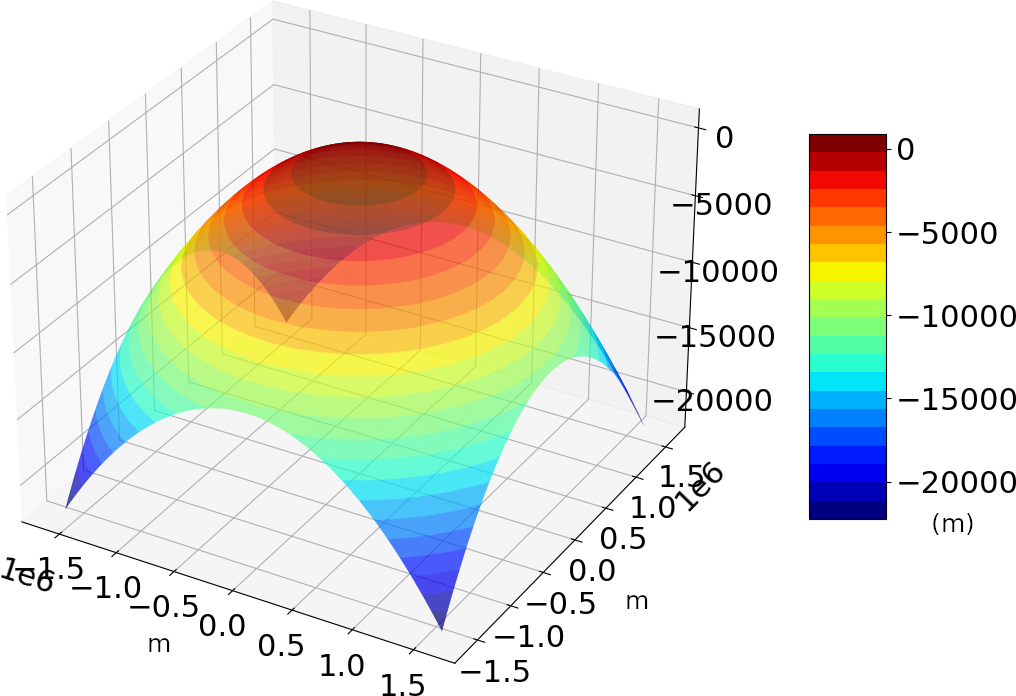
\includegraphics[width=0.7\linewidth]{../fig/circular_topo_jet}
	\caption{Circular bedrock sideview.}
	\label{circular_topo_jet}
\end{figure}
The thule bedrock configuration (Bed) is shown in Figure \ref{Thule_2D} and is given by:
\begin{equation}
	\theta=arctan2(y,x);
\end{equation}
\begin{equation}
	I=R-cos(2\theta)\frac{R}{2};
\end{equation}
\begin{equation}
	Bed_0=Bc-(Bc-BI)\frac{|x^2+y^2}{R^2};
\end{equation}
\begin{equation}
	Bed=Bacos(3\pi\frac{\sqrt[2]{x^2+y^2}}{I})+Bed_0;
\end{equation}
With $R=800 x 10^3 m$, $Bc=0,9 x 10^3 m$, $BI=-2 x 10^3 m$, and $Ba=1,1 x 10^3$.
\begin{figure}[!h]
	\centering
	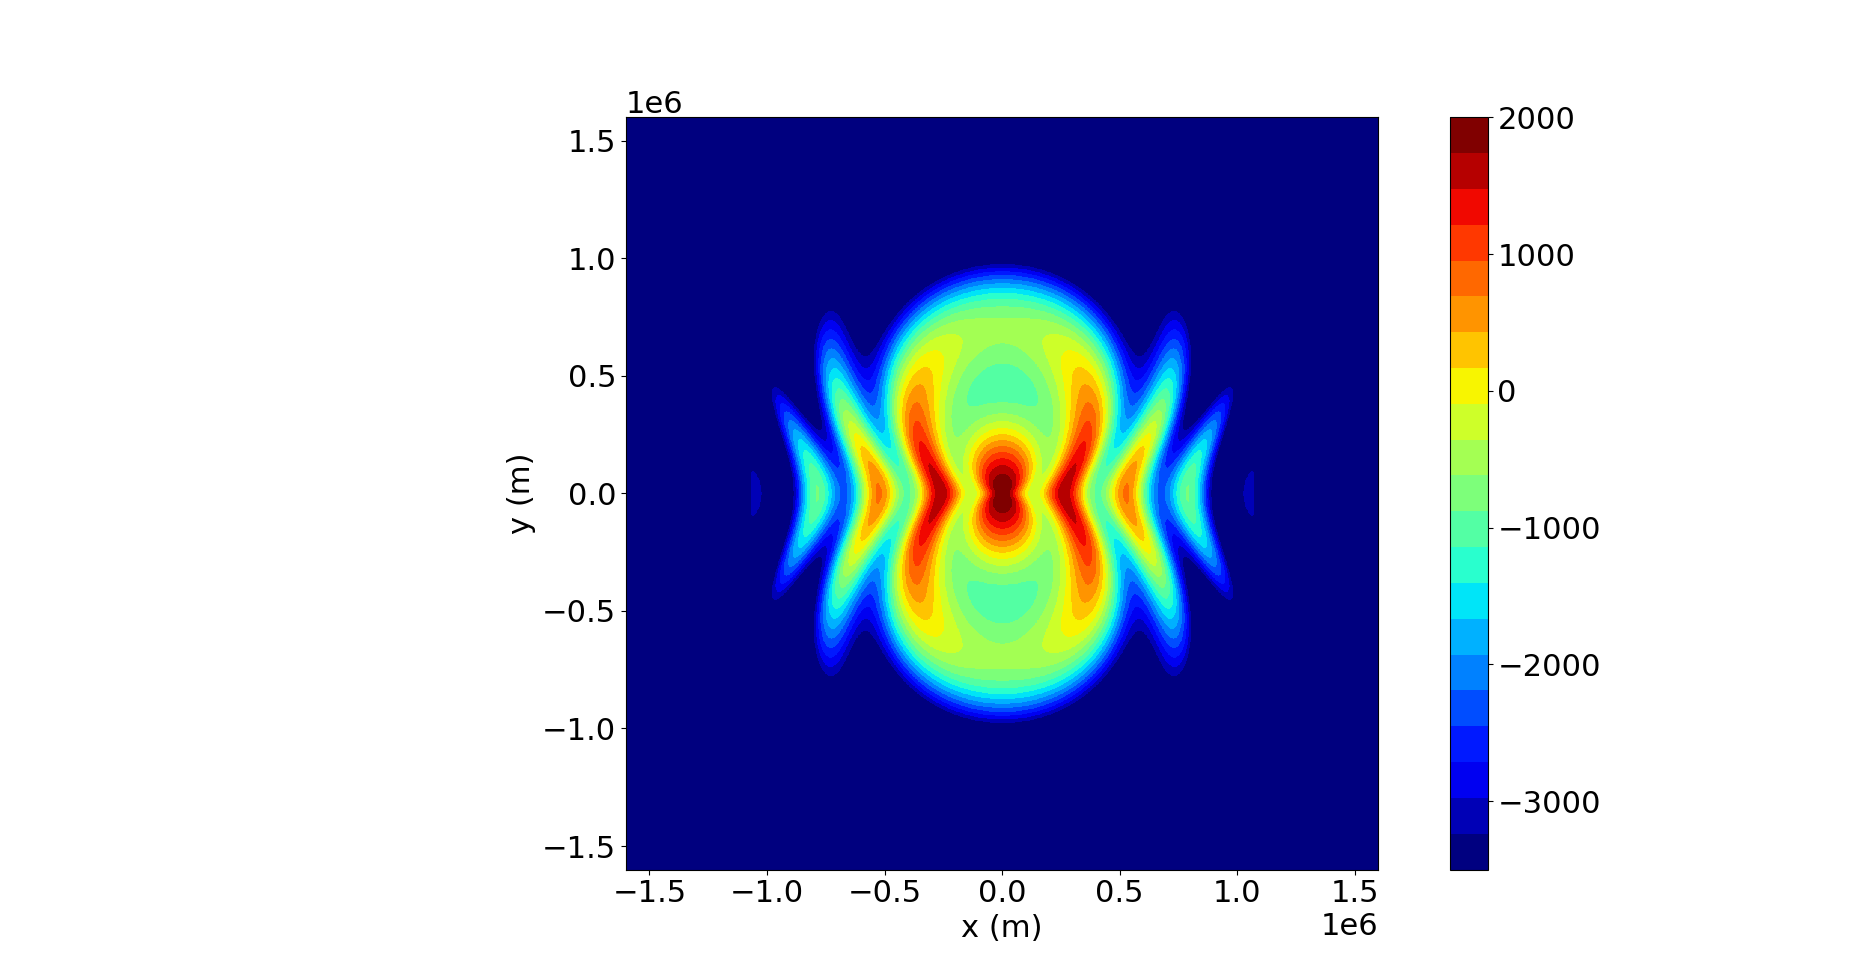
\includegraphics[width=0.7\linewidth]{../fig/Thule_2D}
	\caption{Thule bedrock topview.}
	\label{Thule_2D}
\end{figure}
\begin{figure}[!h]
	\centering
	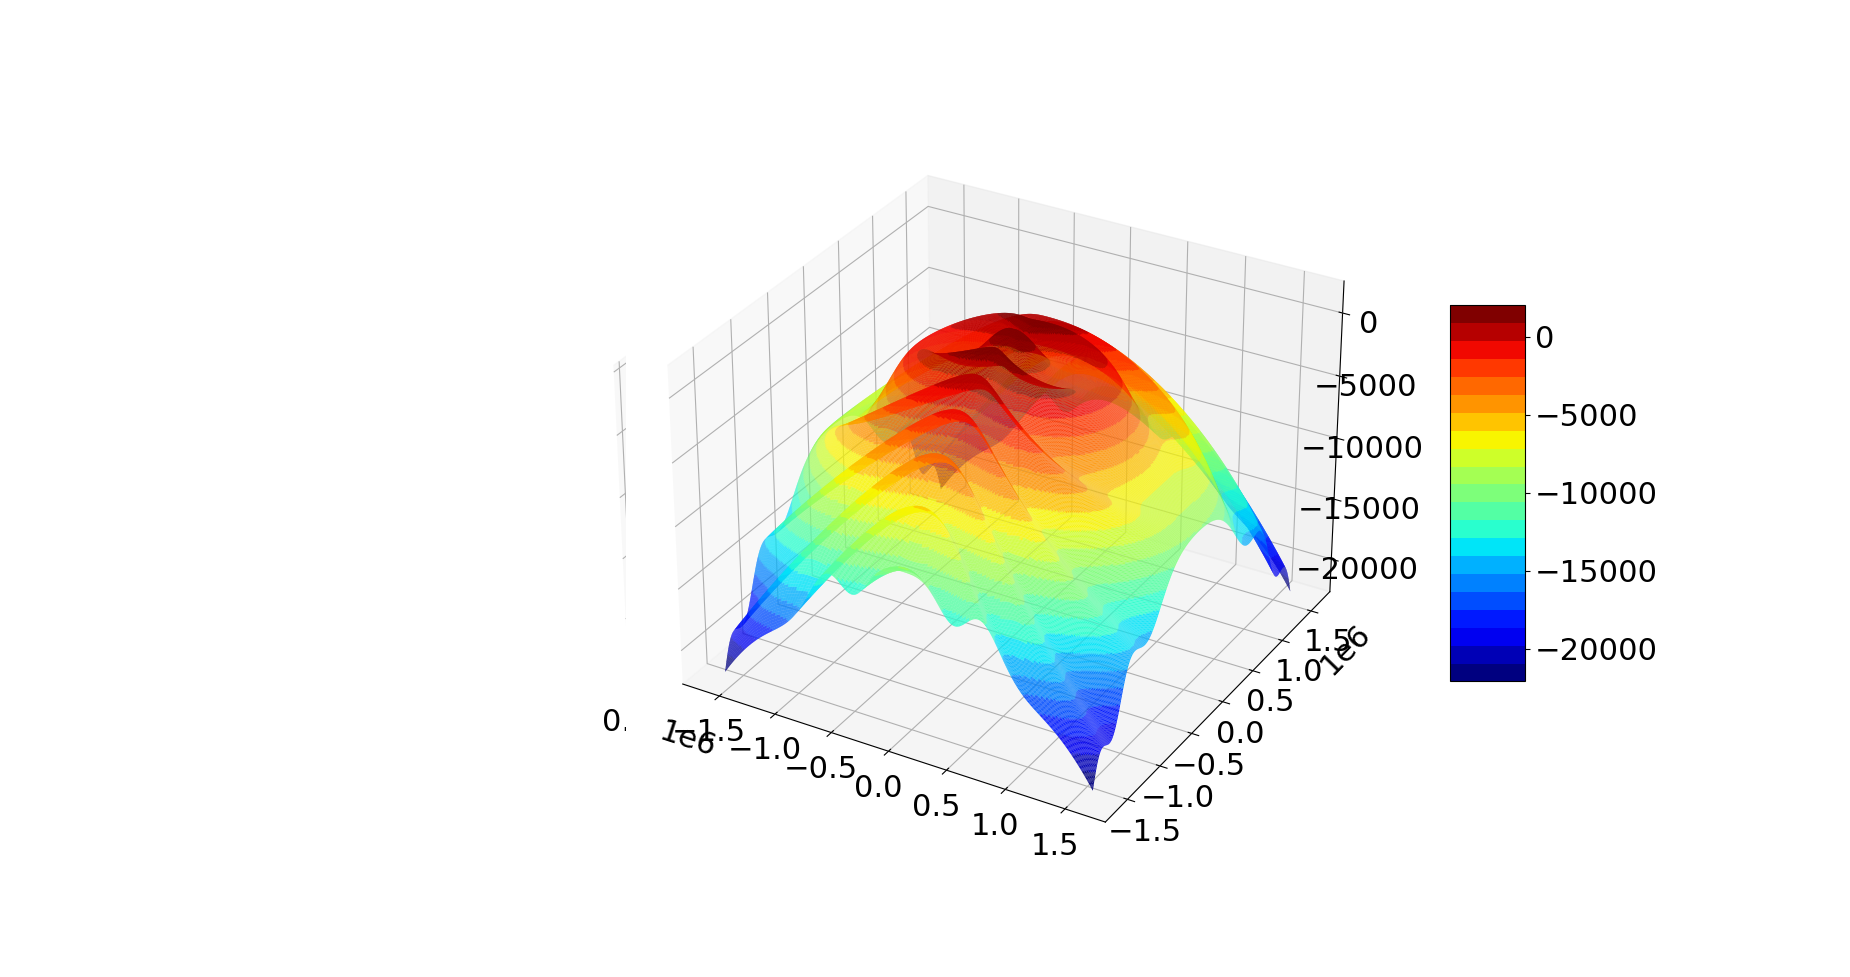
\includegraphics[width=0.7\linewidth]{../fig/Thule_3D}
	\caption{Thule bedrock topography 3D sideview.}
	\label{Thule_3D}
\end{figure}
\subsubsection{Boundary conditions}
Boundary conditions are needed in order to solve differential equations. It will be assumed that:
\begin{itemize}
	\item The bedrock is impermeable (The vertical component of the ice flow velocity is 0). 
	\item The flow follows Weertman friction law.
	\item Mass acumulation is a constant parameter.
	\item The simulation will be performed on a quarter of the domain, since the geometry of the topography is symmetric, which allows to have free slip boundary condition at the left and down side of the topography, and open boundary condition at the right and top side of the domain. 
\end{itemize}
\subsubsection{Physical parameters}
There will be two types of physical parameters in the simulation, the ones we will assume constant during all our simulations, and the ones which can vary during and in between the simulation. The figure \ref{Constants_parameters} presents the constant parameters that will be used
\begin{figure}[!h]
	\centering
	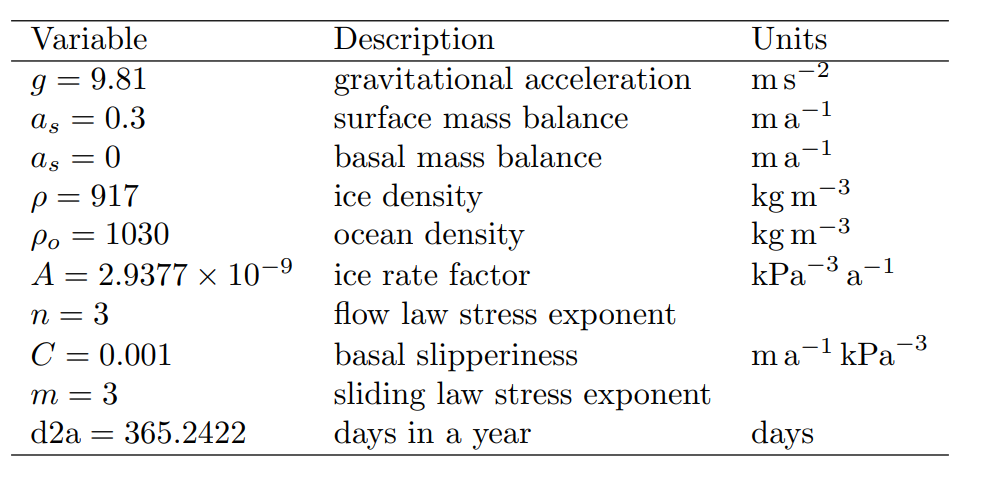
\includegraphics[width=0.7\linewidth]{../fig/Constants_parameters}
	\caption{Constants parameters based on Hilmar Gudmundsson's experiment for thule's configuration.}
	\label{Constants_parameters}
\end{figure}
The numerical resolution will be our variable physical parameter, which we will vary from 10km, 5km, 1km and 500m respectively. 
\subsubsection{External forcing}
We will assume that the only external force acting is the gravity ($g=9.81 m/s^2$), which is translated to the weight of the ice sheet and the flotation force of this in the ocean water.
\subsubsection{Initial condition}
The simulation starts from rest state, were no ice is formed. 
As stated before, the flow will follow the linear Weertman friction law at the base of the ice sheet:
\begin{equation}
	\tau_b=\beta u;
\end{equation}
Where $\tau$ is the friction shear stress, $\beta$ is the basal friction coefficient, and $u$ is the velocity.
Comparisons were made using friction coefficients ranging from $\beta=10^-8$ to simulate a friction close to 0, to $\beta=10^-2$. This coefficient is also the one chosen to perform the simulations. 
\subsubsection{Time step}
The Courant-Friedrichs-Lewy (CFL) condition is a necessary condition to solve numerically partial differential equations. It states that the distance a variable travels between two time steps must be smaller than the distance between two points of the mesh \cite[]{courant1967partial}. It is needed that:
\begin{equation}
	C=\frac{u\Delta t}{\Delta x}<Cmax;
\end{equation}
With C the courant number, $u$ the magnitude of the velocity, $\Delta t$ the time step, $\Delta x$ the horizontal resolution, and Cmax = 1. This implies then, for a given mesh:
\begin{equation}
	\Delta t < \frac{\Delta x}{u};
\end{equation}
This is a safe approximation. Cmax then has to be estimated running different parameters in the simulation and see if it converges or not. In order to satisfy the CFL condition, a good starting point is 1 year, since it works propertly and converges even for a resolution of 1km.
However, in this experiment it is asked to report the results every 10 years, and for this reason we will save the results of the simulation with a frequency of 10 years. 
\subsection{Work plan and tasks schedule}
Figure \ref{Schedule} shows the tasks schedule for the project, that will be held between the 12th of january 2023 and the 5th of may 2023. 
\begin{figure}[!h]
	\centering
	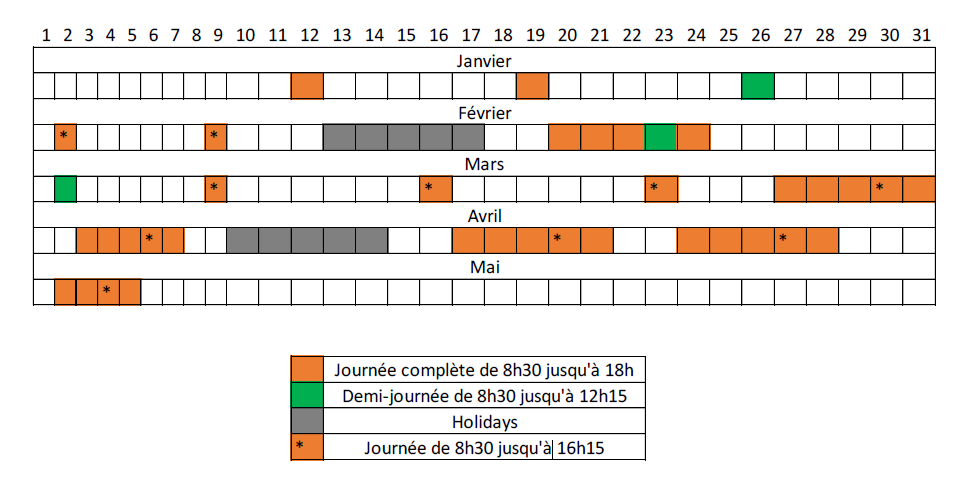
\includegraphics[width=0.7\linewidth]{../fig/Schedule}
	\caption{Tasks schedule of the project, showing the days we will spend working on the different stages of it.}
	\label{Schedule}
\end{figure}
During February, we will run the idealised simulations. As a starting point we will do it using 10 km, 5km, 1km, and 500m resolutions. The simulations take around 1 day, 2 days, 5 days, and 1 week, respectively. This means that, according to the schedule, we will have the simulations results by the last week of February. 

In March, we will proceed with the data analysis of the results we obtained from all the idealised simulations. During the first week of April, and according to the results obtained, we may study a different case or configuration with a different resolution, mesh or parameter; and the rest of the month we will write and proceed with the complementary studies. At last, during the first week of may we will work on the presentation of the results/conclutions of the experiments. 
\bibliographystyle{jfm}
\bibliography{./biblio}
\end{document}
